\documentclass{beamer}
\usetheme{Madrid}
\usecolortheme{beaver}
%\usepackage{graphicx}
%\graphicspath{{img/}}
\usepackage{color}
\usepackage[utf8]{inputenc}
\usepackage{graphicx}
\usepackage[spanish]{babel}
\usepackage{booktabs}
\usepackage{background}
\setbeamertemplate{navigation symbols}{}%remove navigation symbols

%\backgroundsetup{
%	placement=center,
%	scale=1.5,
%	contents={Versión preliminar- no circular},
%	opacity=1}
%\setbeamertemplate{background}{\BgMaterial}

\title[Imputación usando Ensamble Learning]{Maximizando el ROI de los datos mediante Imputación de valores perdidos con \emph{Ensamble Learning}}
\author{Germán Rosati \\ \href{mailto: german.rosati@gmail.com}{german.rosati@gmail.com}}
%\institute[Digital House]{Programa de Ciencia de Datos- Digital House}
\institute{UNTREF / MTEySS / Digital House}
\date{26 de Abril de 2017}
%\logo{\includegraphics[height=0.4cm]{img/header-logo.png}}

\begin{document}
\frame{\titlepage}

%\begin{frame}
%	\frametitle{Hoja de ruta}
%	\tableofcontents
%\end{frame}

\section{Introducción}
\begin{frame}
	\frametitle{Hoja de ruta}
	\begin{enumerate}
		\item{¿Qué es y como se genera un dato perdido?}
		\item{¿Cómo lidiar con los datos perdidos?}
		\begin{itemize}
			\item{Técnicas tradicionales (imputación simpe)}
		\end{itemize}
		\item{Ejercicio de aplicación}
	\end{enumerate}
\end{frame}

\begin{frame}
	\begin{center}
		{\huge ¿Qué es un dato perdido?
			\linebreak
			\linebreak
			\linebreak
			\linebreak}
	\end{center}
\end{frame}

\section{¿Qué es un valor perdido?}
\begin{frame}
	\frametitle{¿Qué es un valor perdido?}
	\begin{itemize}
		\item{Los datos son caros}
		\begin{itemize}
			\item{Encuestas}
			\item{SRMs}
			\item{Logs, Analytics}
			\item{Sistemas de Web Scrapping}
		\end{itemize}
		\item{Los datos son muchos}
		\item{Los datos están sucios}
		\begin{itemize}
			\item{Inconsistencias}
			\item{Errores en la carga, escritura}
			\item{Valores faltantes}
			\item{No respuestas totales o parciales}
		\end{itemize}
		\item{Cualquier error impacta en el valor que podemos extrear de un dataset}
	\end{itemize}
\end{frame}
	 

\begin{frame}
\frametitle{¿Qué es un valor perdido?}
	\begin{itemize}
		\item{Valor del que se carece una dato válido en la variable observada}
		\item{Problema generalizado en investigaciones por encuestas}
		\item{Problema cada vez más frecuente en investigaciones que usan registros administrativos o datos de redes sociales, aplicaciones, etc.}
		\item{¿Cómo se generan esos datos perdidos?}
	\end{itemize}
\end{frame}

\section{Procesos generadores de valores perdidos}
\subsection{MCAR}
\begin{frame}
	\frametitle{Procesos de generación de valores perdidos}
	\framesubtitle{Missing Completely at Random -MCAR-}
	\begin{itemize}
		\item{La probabilidad de que registro tenga un valor perdido en la variable $Y$ no está relacionada ni con los valores de $Y$, ni con otros valores de la matriz de datos ($X$)}
		\item{Los valores perdidos son una submuestra al azar de los valores totales}
		\item{¿Cuándo no hay MCAR?}
			\begin{enumerate}
			\item{Si algún grupo tiene mayor probabilidad de presentar datos perdidos en la variable $Y$ y/o} 
			\item{si alguno de los valores de $Y$ tiene mayor probabilidad de presentar datos perdidos}
			\end{enumerate}

	\end{itemize}
\end{frame}

\subsection{MAR-MNAR}
\begin{frame}
	\frametitle{Procesos de generación de valores perdidos}
	\framesubtitle{Missing at Random -MAR- y Missing Not at Random -MNAR-}
	\begin{itemize}
		\item{\textbf{MAR:} La probabilidad de no respuesta en $Y$ es independiente de los valores de $Y$, luego de condicionar sobre otras variables}
		\item{\textbf{MNAR:} La probabilidad de no respuesta depende tanto de variables $X$ externas, como de los valores de la variable con datos perdidos ($Y$)}
	\end{itemize}
\end{frame}

\begin{frame}
	\frametitle{Procesos de generación de valores perdidos}
	\framesubtitle{Resumen}
	\begin{figure}
		\centering
		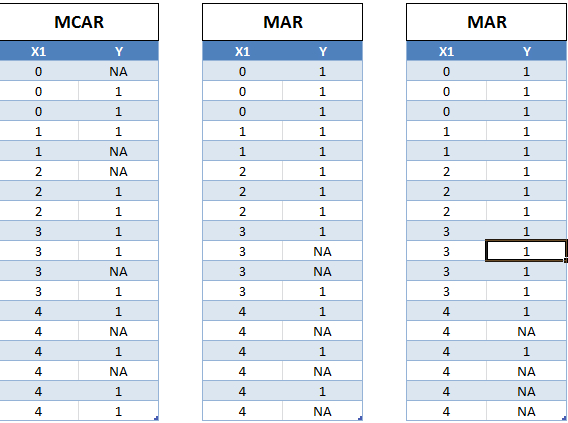
\includegraphics[width=0.55\linewidth, height=0.66\textheight]{img/2_patterns}
		%\caption{Esquema de procesos de generación de datos perdidos}
		%\label{fig:2_patterns}
\end{figure}
\end{frame}

\begin{frame}
	\frametitle{¿Por qué es importante imputar datos?}
	\framesubtitle{Un ejemplo: EPH}
	\small{\textbf{Proporción de casos imputados (sin datos en alguna variable de ingresos) en EPH. Total de aglomerados urbanos, 2003-2015 (II-Trimestre de cada año)}}
	\begin{figure}
		\centering
		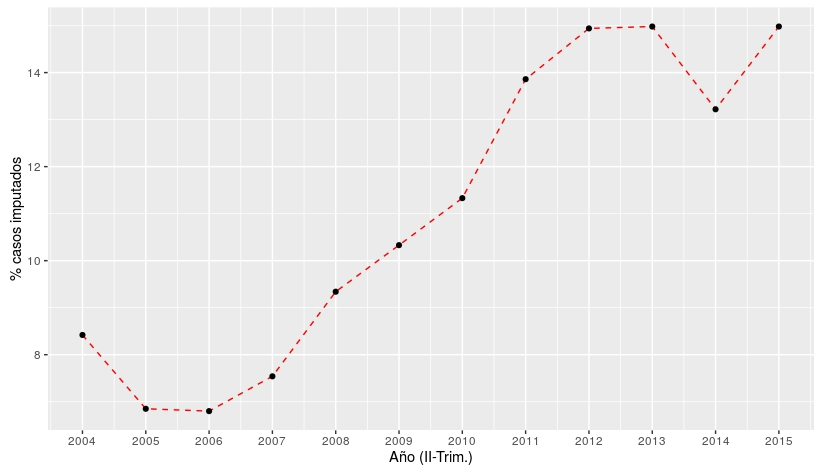
\includegraphics[width=0.7\linewidth, height=0.55\textheight]{img/4_ehp_NR}
	\end{figure}
\end{frame}

\begin{frame}
	\begin{center}
		{\huge ¿Cómo lidiar con los datos perdidos?
			\linebreak
			\linebreak
			\linebreak
			\linebreak}
	\end{center}
\end{frame}

\section{¿Cómo lidiar con valores perdidos?}
\subsection{Métodos de Imputación Simple}

\begin{frame}
	\frametitle{¿Cómo lidiar con valores perdidos?}
	\framesubtitle{Imputación simple}
		\begin{itemize}
			\item{\textbf{Excluir los casos:} se trabaja solamente con los casos completos en toda la base o solamente en las variables de estudio. Problema: se achica el dataset.}
			\item{\textbf{Reemplazar por la media o alguna otra medida:} Problema: reducción de la variabilidad de la información y se generan intervalos de confianza más estrechos de forma artificial.}
			\item{\textbf{Reponderación:} se recalculan los ponderadores de la muestra (a partir de algoritmos de reweighting) para compensar el efecto de los casos con información faltante. Problema: es incómodo trabajar con varios sets de pesos.}
			
		\end{itemize}
\end{frame}

\begin{frame}
	\frametitle{¿Cómo lidiar con valores perdidos?}
	\framesubtitle{Métodos de imputación simple - Hot Deck}
	\begin{itemize}
		\item{Método ampliamente usado. INDEC -hasta 2015- y Dirección de Estadística de la Ciudad para realizar imputaciones en EPH y EAH}
		\item{Reemplazar valores perdidos de un no respondente (“receptor”) con los valores observados de un respondente (“donante”) que es similar al receptor.}
	\end{itemize}
\end{frame}

\begin{frame}
	\frametitle{¿Cómo lidiar con valores perdidos?}
	\framesubtitle{Métodos de imputación simple - Hot Deck}
	\begin{itemize}
		\item{\textbf{Problema 1:} selección de la "métrica" de similitud entre los casos}
		\item{\textbf{Problema 2:} selección de los donantes}. {El donante es seleccionado aleatoriamente de un set de potenciales donantes –hot-deck aleatorio- o bien se selecciona un solo caso donante, generalmente a partir de un algoritmo de “vecinos cercanos” usando alguna métrica -hot-deck determinístico-.}
	\end{itemize}
\end{frame}

\subsection{Técnicas de Ensamble Learning}
\begin{frame}
	\frametitle{¿Cómo lidiar con valores perdidos?}
	\framesubtitle{Ensamble Learning}
	\begin{columns}
		\begin{column}{0.48\textwidth}
			\begin{itemize}		
					\item Técnicas de aprendizaje supervisado donde se combinan varios modelos base.
					\item Ampliar el espacio de hipótesis posibles para mejorar la precisión predictiva del modelo combinado resultante.
					\item Los ensambles suelen ser mucho más precisos que los modelos base que los componen.
			\end{itemize}
		\end{column}
		\begin{column}{0.85\textwidth}
			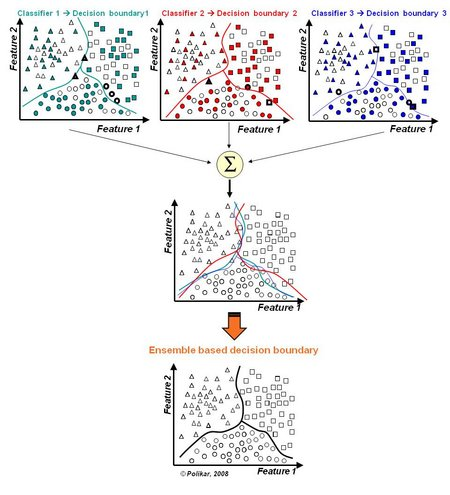
\includegraphics[width=0.657\linewidth, height=0.7\textheight]{img/ensamble.jpg}
		\end{column}
	\end{columns}
\end{frame}

\subsubsection{Bagging}
\begin{frame}
	\frametitle{¿Cómo lidiar con valores perdidos?}
	\framesubtitle{Ensamble Learning - Bagging}
	\begin{columns}
		\begin{column}{0.48\textwidth}
	\begin{itemize}		
		\item Construcción de estimadores independientes -Boostrap-
		\item  Combinación las predicciones mediante función agregación. 
		\item Ejemplos: Random Forest, ExtraTrees, etc.
	\end{itemize}
		\end{column}
		\begin{column}{0.85\textwidth}
			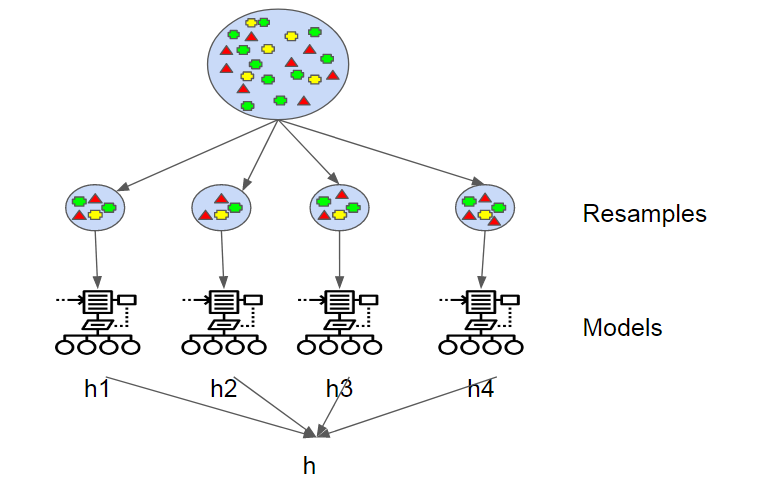
\includegraphics[width=0.7\linewidth, height=0.7\textheight]{img/bagging}
		\end{column}
	\end{columns}
\end{frame}

\subsubsection{Boosting}
\begin{frame}
	\frametitle{¿Cómo lidiar con valores perdidos?}
	\framesubtitle{Ensamble Learning - Boosting}
	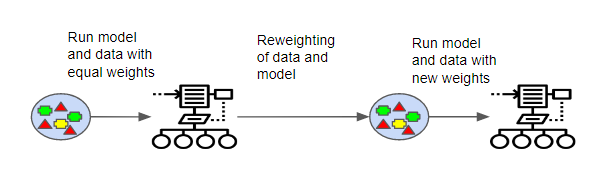
\includegraphics[width=1\linewidth, height=0.5\textheight]{img/boosting}
	\begin{itemize}		
		\item Construcción secuencial de los estimadores 
		\item Mayor peso en aquellos casos en los que se observa una peor performance. 
		\item Ejemplos: AdaBoost y Gradient Tree Boosting, XGBoost.
	\end{itemize}
\end{frame}

\subsection{Aplicación a un caso real: EPH}
\subsubsection{Random Forest}
\begin{frame}
	\frametitle{¿Cómo lidiar con valores perdidos? - Método posible 1}
	\framesubtitle{Ensamble Learning - Random Forest}
	\begin{columns}
		\begin{column}{0.48\textwidth}
			\begin{itemize}		
				\item Variación del algoritmo Bagging
				\item Modelo base: árboles de decisión
				\item Feature Bagging, en cada iteración y en cada split del árbol de decisión, el algoritmo selecciona aleatoriamente un subconjunto de variables predictoras
			\end{itemize}
		\end{column}
		\begin{column}{0.85\textwidth}
			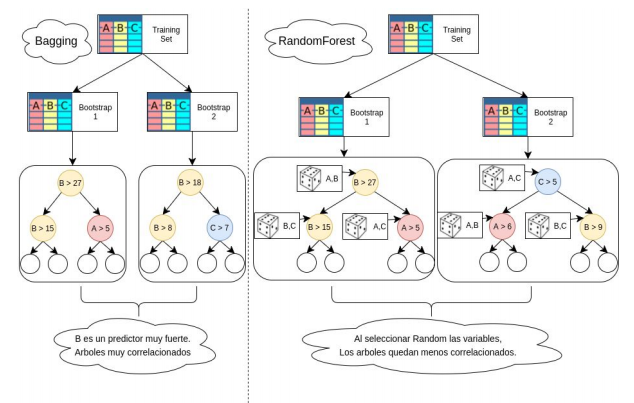
\includegraphics[width=0.67\linewidth, height=0.6\textheight]{img/random_forest}
		\end{column}
	\end{columns}
\end{frame}

\begin{frame}
	\begin{center}
		{\huge Un ejercicio de aplicación
			\linebreak
			\linebreak
			\linebreak
			\linebreak}
	\end{center}
\end{frame}

\begin{frame}
	\frametitle{LAB: Imputando datos perdidos con Random Forest}
	\begin{itemize}		
		\item Dataset: EPH 2do. trimestre de 2015
		\item Población: Ocupados en la semana de referencia
		\item Objetivo: Generar un imputador de la variable ingresos
		\item{Variables predictoras sociodemográficas, laborales y otros ingresos}
		\item Pipeline
		\begin{enumerate}
		\item Partición Train-Test
		\item Sobre Train: entrenamos un clasificador Random Forest
		\item Sobre Train: entrenamos dos imputadores Hot-Deck
		\item Sobre Test: evaluamos los resultados
		\end{enumerate}
	\end{itemize}
\end{frame}

\subsubsection{Bagging-LASSO}
\begin{frame}
	\frametitle{¿Cómo lidiar con valores perdidos? - Método posible 2}
	\framesubtitle{Bagging-LASSO}
	\centering
	
\includegraphics[width=0.7\linewidth, height=0.7\textheight]{img/saberes}

\end{frame}

\begin{frame}
\frametitle{¿Cómo lidiar con valores perdidos? - Método posible 2}\subsection{Técnicas de Ensamble Learning}
\framesubtitle{Bagging-LASSO}
	\begin{itemize}
		\item{Se aplica el algoritmo bagging a la imputación de ingresos laborales en la EPH del II trimestre de 2015}
		\item{En cada remuestra se estima la siguiente regresión LASSO}
		\begin{equation}
		log_{10}(y_{i}) = \beta_{0} + \sum_{j=1}^pX_{ij}\beta_{j} + e_{i}
		\end{equation}
		\item{Buscando minimizar la siguiente función de costo:}
		\begin{equation}
		CF = RSS + \lambda\sum_{j=1}^p|\beta_{j}|
		\end{equation}
	\end{itemize}
\end{frame}

\begin{frame}
\frametitle{¿Cómo lidiar con valores perdidos? - Método posible 2}
\framesubtitle{Bagging-LASSO}
	\begin{enumerate}
		\item Se crea un dataset con todos los casos completos\emph{TrS}
		\item Se crea otro dataset con los casos son datos perdidos \emph{TeS} 
		\item Se fija la cantidad de iteraciones \emph{rep}
		\item Para $r$ entre 1 y \emph{rep}
		\begin{enumerate}
			\item Se extrae una muestra boostrap (MAS con reemplezo y $n=n^*$) de \emph{TrSet}
			\item En la muestra generada se estima una regresión LASSO
			\item Con los parámetros estimados en el paso anterior se realiza la predicción en el \emph{TeS}
		\end{enumerate}
		\item Luego de \emph{rep} iteraciones se generan \emph{rep} predictiones de los casos perdidos en \emph{TeS} y se agregan usando la mediana
	\end{enumerate}					
\end{frame}


\begin{frame}
\frametitle{¿Cómo lidiar con valores perdidos? - Método posible 2}
\framesubtitle{Bagging-LASSO}
\begin{itemize}
	\item{Generación de datos perdidos de forma aleatoria}
	\item{Para evaluar performance de Bagging-LASSO y hot-deck se estima el $RMSE$ a través de \emph{k-fold cross validation}, con $k=9$}
	\begin{enumerate}
		\item{$RMSE-LASSO = 3.994\$$}
		\item{$RMSE-hot deck = 4.933\$$}
	\end{enumerate}
	\item{Es decir, una reducción de alrededor del 20\%}
	\item{La imputación Bagging-LASSO mejora considerablemente el error de predicción de los ingresos laborales}
	\item{Esperable que en datos perdidos “originales” (es decir, no generados 		artificialmente) el método consiga una mejor performance que hot-deck}
\end{itemize}
\end{frame}

\section{Resumen y Resultados}
\begin{frame}
	\frametitle{Resumen}
	\begin{itemize}
		\item Procesos generadores de datos perdidos
		\item Técnicas "tradicionales"
		\item Ensamble Learning como alternativa
		\item Random Forest logra una reducción considerable en el $RMSE$ entre casos perdidos comparado a Hot Deck
		\item Baggin-LASSO también logra una mejora sustantiva
	\end{itemize}
\end{frame}

\begin{frame}
	\begin{center}
	{\huge ¿Preguntas?
		\linebreak
		\linebreak
		\linebreak
		\linebreak}
	{\Large
		\color{blue}
		german@digitalhouse.com \linebreak
		german.rosati@gmail.com
	}
	\end{center}
\end{frame}
	
\end{document}